\documentclass[11pt]{article}

\usepackage[margin=1.2in]{geometry}
\usepackage{booktabs}
\usepackage{graphicx}
\usepackage{hyperref}
\usepackage{amsmath}
\usepackage{array}
\usepackage{float}
\setlength{\parskip}{6pt}
\setlength{\parindent}{0pt}

\hypersetup{colorlinks=true, linkcolor=black, urlcolor=blue, citecolor=black}

\title{Mantis IP Visualization: RAG Retrieval Pipelines\\
\large Standard retrieval, IPC-weighted scoring, and long-document chunking}
\author{Mantis IP Visualization}
\date{July 2026}

\begin{document}
\maketitle
\tableofcontents
\newpage

% ─────────────────────────────────────────────────────────────────────────────
\section{Introduction}
% ─────────────────────────────────────────────────────────────────────────────

This document covers the retrieval tooling I build using The Lens Patent Corpus sample dataset (\texttt{lens-db-translated.json}, roughly 7,400 English-language patent records after
filtering for non-empty title and abstract fields). The goal with these methods was to take a given query document/input and return a ranked list of the most relevant patents in the corpus. The core problem is that these inputs are diverse in both size and type (e.g. some inputs contain IPC codes, some are 1,000+ words, etc.). As such, there are 3 different pipelines in this repository. The first tests multiple standard RAG systems, the second incorporates IPC-classifying codes into the final document relevancy score. The third one uses document chunking to handle documents too long for one pass. All of
the code referenced here is in the \texttt{rag-testing/} directory of the project
GitHub repository.

% ═════════════════════════════════════════════════════════════════════════════
\part{standard-rag/: baseline retrieval comparison}
% ═════════════════════════════════════════════════════════════════════════════

% ─────────────────────────────────────────────────────────────────────────────
\section{Goal}
% ─────────────────────────────────────────────────────────────────────────────

Which retrieval method gives the best relevance per millisecond over the patent
corpus? To answer this, I built three retrieval systems and tested them on the same
nine test queries. These queries included patent abstracts, product descriptions of
different lengths, and plain-language queries of different lengths.

\begin{itemize}
  \item \textbf{BM25} is a classic sparse lexical retrieval method. It scores
    documents using term-frequency and inverse-document-frequency statistics over
    tokenized title and abstract text. It does not use an embedding model.
  \item \textbf{MiniLM} is a dense retrieval method. It uses \texttt{all-MiniLM-L6-v2},
    a small general-purpose sentence-embedding model.
  \item \textbf{BGE-small} is a dense retrieval method. It uses
    \texttt{BAAI/bge-small-en-v1.5}, a model built specifically for retrieval. It adds
    an instruction prefix (\texttt{"Represent this sentence for searching relevant
    passages: "}) to the query text only, not to the corpus text.
\end{itemize}

For both dense methods, I L2-normalize the corpus embeddings when I build the index.
This means cosine similarity becomes a simple dot product at query time, which is
faster to compute. This is also why the embeddings cache
(\texttt{*\_embeddings.npy}) stores normalized vectors instead of raw ones.

% ─────────────────────────────────────────────────────────────────────────────
\section{Setup and reused signal}
% ─────────────────────────────────────────────────────────────────────────────

All three systems index the same text for each patent: the title and abstract
combined. I embed or tokenize this text once and cache the result to disk
(\texttt{results/bm25/}, \texttt{results/minilm/}, and \texttt{results/bge/}). This
means repeat queries do not need to rebuild the index. The query times reported
below measure only the score computation step. They do not include model or index
load time.

% ─────────────────────────────────────────────────────────────────────────────
\section{Results}
% ─────────────────────────────────────────────────────────────────────────────

\begin{figure}[H]
  \centering
  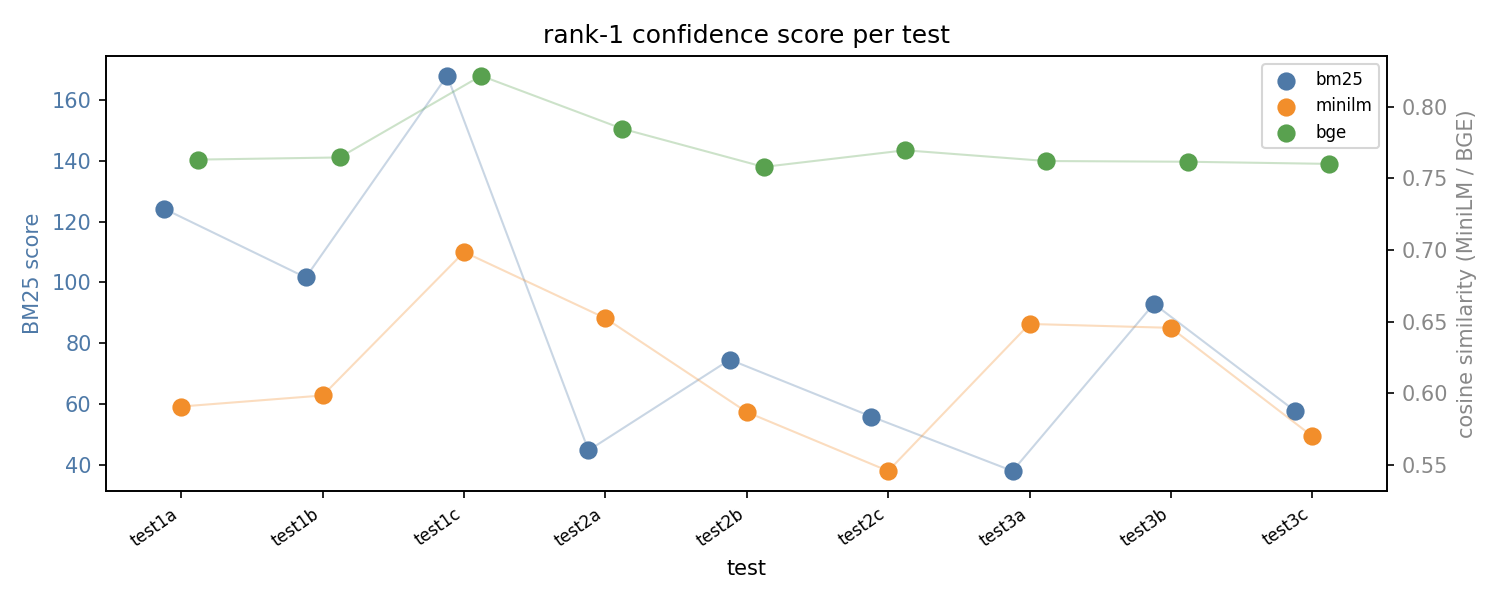
\includegraphics[width=\textwidth]{standard-rag/results/statistics/fig1_scores.png}
  \caption{Rank-1 confidence score per test query. BM25 scores (left axis) are
  unbounded term-frequency scores. MiniLM and BGE scores (right axis) are cosine
  similarities in $[0,1]$. BGE's top score stays in the 0.75 to 0.82 range across
  every test. It is the flattest of the three lines, so it is the least sensitive
  to changes in query phrasing or length.}
\end{figure}

\begin{figure}[H]
  \centering
  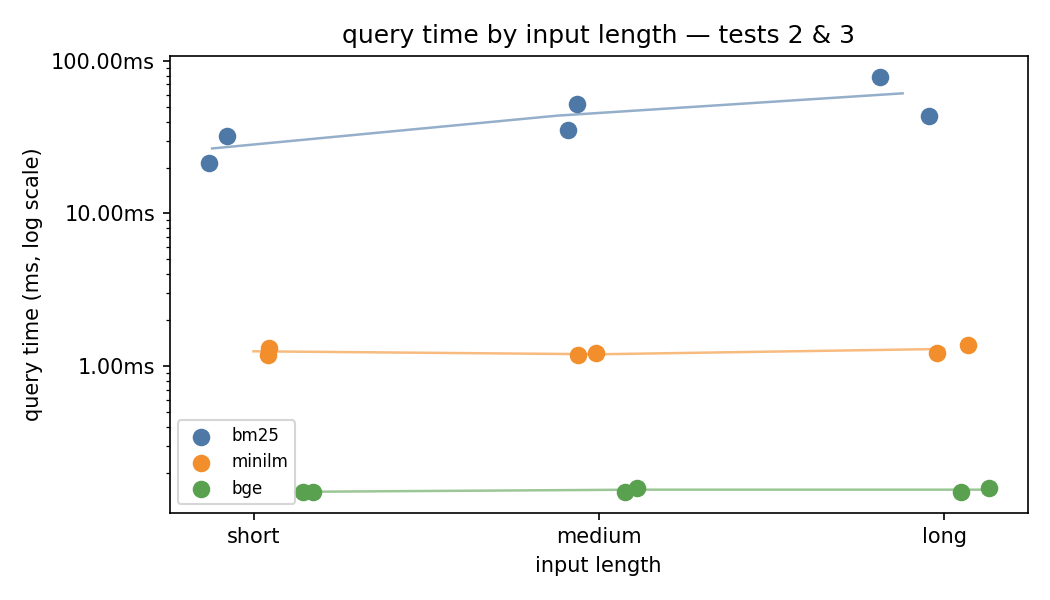
\includegraphics[width=0.85\textwidth]{standard-rag/results/statistics/fig2_times.png}
  \caption{Query time by input length (log scale), tests 2 and 3. BGE is roughly
  two orders of magnitude faster per query than BM25 and stays flat as input length
  grows, since the entire query is reduced to one embedding regardless of length.}
\end{figure}

\begin{center}
\small
\begin{tabular}{lccc}
  \toprule
  \textbf{Metric} & \textbf{BM25} & \textbf{MiniLM} & \textbf{BGE-small} \\
  \midrule
  Query time (typical) & 20 to 80\,ms & 1 to 3\,ms & 0.15 to 0.17\,ms \\
  Rank-1 score (mean, tests 1 to 3) & about 87 (unbounded) & about 0.62 & about 0.78 \\
  Query-time scaling with input length & grows (roughly linear) & flat & flat \\
  Short-vs-long overlap, Jaccard (top-10) & 0.25 to 0.43 & 0.33 to 0.43 & 0.25 \\
  \bottomrule
\end{tabular}
\end{center}

\textbf{Takeaway:} I chose BGE-small as the retrieval backbone for the two downstream
pipelines, \texttt{code-weight/} and \texttt{longdoc-rag/}. It has the fastest query
time of the three methods by a wide margin. It also has the highest and most stable
rank-1 confidence scores. On top of that, it is a dense method with normalized
embeddings, so it fuses cleanly with additional signal. That fusion is exactly what
the IPC-weighting pipeline below needs.

% ═════════════════════════════════════════════════════════════════════════════
\part{code-weight/: IPC-weighted retrieval}
% ═════════════════════════════════════════════════════════════════════════════

% ─────────────────────────────────────────────────────────────────────────────
\section{Goal}
% ─────────────────────────────────────────────────────────────────────────────

Patent records carry IPC (International Patent Classification) codes. These codes
form a hierarchical taxonomy assigned by patent examiners, and they are a
human-curated relevance signal that is arguably stronger than free text alone. A
pure text-embedding retrieval system throws this signal away entirely. My goal with
this pipeline is to combine semantic text similarity with IPC-taxonomy similarity.
Two patents in the same narrow classification should rank higher relative to each
other than raw cosine similarity alone would suggest. At the same time, the system
should still fall back to plain semantic search when IPC codes are missing or not
useful.

% ─────────────────────────────────────────────────────────────────────────────
\section{IPC taxonomy and scoring}
% ─────────────────────────────────────────────────────────────────────────────

An IPC code such as \texttt{C07H21/04} breaks down into five hierarchical levels.
Each level is more specific than the one before it:

\begin{center}
\small
\begin{tabular}{lll}
  \toprule
  \textbf{Level} & \textbf{Example} & \textbf{Meaning} \\
  \midrule
  Section    & C          & Top-level domain (Chemistry and Metallurgy) \\
  Class      & C07        & Organic chemistry \\
  Subclass   & C07H       & Sugars, nucleosides, nucleotides \\
  Main group & C07H21     & Compounds containing nucleoside/nucleotide units \\
  Subgroup   & C07H21/04  & Full code, specifically deoxyribonucleic acids \\
  \bottomrule
\end{tabular}
\end{center}

For a pair of IPC codes, I score their similarity based on the \textbf{deepest level
at which they agree}:

\begin{center}
\small
\begin{tabular}{lc}
  \toprule
  \textbf{Deepest matching level} & \textbf{Score} \\
  \midrule
  Subgroup (full code match)   & 1.0 \\
  Main group                   & 0.8 \\
  Subclass                     & 0.5 \\
  Class                        & 0.2 \\
  Section only, or no match    & 0.0 \\
  \bottomrule
\end{tabular}
\end{center}

A query usually carries several IPC codes, and so does each corpus document. To
score a document, I look at every pair of a query code and a document code, and I
take the \textbf{maximum} score across all of those pairs. This means a document
only needs one strong classification match with the query to score well. It does
not matter if its other codes are unrelated.

% ─────────────────────────────────────────────────────────────────────────────
\section{Fusion with semantic score}
% ─────────────────────────────────────────────────────────────────────────────

Before combining the two scores, I first min-max normalize the BGE cosine similarity
across the whole corpus for the current query. This puts it in the same $[0,1]$
range as the IPC score. Without this step, the IPC term would unfairly dominate,
since cosine scores are usually compressed into a narrow band between 0.55 and 0.85,
while IPC scores are spread across the full range. The final score is a weighted sum
of the two:

\[
  \text{Score}_{\text{final}} = \alpha \cdot \text{cos}_{\text{norm}} + (1-\alpha) \cdot \text{IPC}_{\text{score}}
\]

I use $\alpha = 0.7$. This gives 70 percent weight to the semantic score and 30
percent weight to the IPC score. If a document has no IPC codes at all, I drop the
IPC term and the score falls back to normalized cosine alone. This way, patents
without IPC codes are never unfairly penalized.

% ─────────────────────────────────────────────────────────────────────────────
\section{Validation: clean vs.\ dirty IPC inputs}
% ─────────────────────────────────────────────────────────────────────────────

I wanted to confirm that the IPC term was actually moving rankings, rather than just
sitting there without doing anything. To test this, I ran every test query twice
while keeping the query text fixed. The first run used the real, semantically
relevant IPC codes (\texttt{inputs-clean/}). The second run used IPC codes sampled
from an unrelated technology area instead (\texttt{inputs-dirty/}).

For the biotech test query (\texttt{test1a}), the clean run used codes
\texttt{A61K9/51}, \texttt{A61K48/00}, and \texttt{A61P35/00}. These codes cover drug
delivery, gene therapy, and antineoplastic activity. The dirty run swapped in
unrelated codes from automotive, construction, and mechanical domains instead
(\texttt{B62D25/08}, \texttt{E04B1/00}, and \texttt{F16H57/00}). Here is the effect
on the top result:

\begin{center}
\small
\begin{tabular}{lccc}
  \toprule
  \textbf{Variant} & \textbf{Rank-1 doc} & \textbf{cos\_norm} & \textbf{IPC score / final} \\
  \midrule
  Clean & mRNA tumor-suppressor delivery system & 1.00 & 1.0 / \textbf{1.00} \\
  Dirty & (same doc, now ranked \#2) & 1.00 & 0.0 / \textbf{0.70} \\
  \bottomrule
\end{tabular}
\end{center}

With clean IPC codes, the document with a perfect classification match gets pulled
up to rank 1. This happens even though it does not have the single highest raw
cosine score in the set. With dirty codes, that same document's IPC term collapses
to 0.0, since it has no overlap with the unrelated taxonomy. Its final score drops
from 1.00 to 0.70, and a different document takes rank 1 instead. That other
document has no IPC codes, so it falls back to cosine-only scoring. This confirms
that the fusion term has a real, correctly-directed effect on the ranking. It is not
just a no-op.

% ═════════════════════════════════════════════════════════════════════════════
\part{longdoc-rag/: chunked retrieval for long documents}
% ═════════════════════════════════════════════════════════════════════════════

% ─────────────────────────────────────────────────────────────────────────────
\section{Goal}
% ─────────────────────────────────────────────────────────────────────────────

Real patent applications and technical filings often run to thousands of words. This
is far beyond BGE-small's 512-token input limit. If I embed the whole document in
one pass, one of two bad things happens. Either the document gets truncated, which
silently throws away content past the limit, or many unrelated sections get blurred
into a single vector that does not represent any of them well. This pipeline solves
that problem for long plain-text query documents. It splits a document into
overlapping chunks, scores each chunk against the corpus on its own, and then
combines the per-chunk scores into one ranked list per corpus document.

% ─────────────────────────────────────────────────────────────────────────────
\section{Chunking methodology}
% ─────────────────────────────────────────────────────────────────────────────

\textbf{Tokenizer.} I tokenize the document using BGE-small's own tokenizer, accessed
through \texttt{model.tokenizer}. I do not use a generic word splitter. Chunk
boundaries need to be counted in the same units the model will actually truncate on.

\textbf{Chunk size.} Each chunk is 300 tokens long. This sits comfortably under
BGE-small's 512-token limit.

\textbf{Overlap.} Consecutive chunks share 15 percent of the chunk size. This way, a
sentence or fact that falls on a chunk boundary still appears intact in at least one
chunk. This overlap gives a \textbf{stride}, which is how far the window moves
forward each step. The stride is roughly $0.85 \times 300 \approx 255$ tokens.

\textbf{Sliding window.} The first chunk covers tokens $[0, 300)$. The second chunk
covers tokens $[255, 555)$. Each following chunk starts where the stride places it,
and this continues until the document is covered.

\textbf{Tail handling.} If the tokens left over are fewer than the chunk size, I
take them as-is for the final chunk. I do not pad them, and I stop there.

\textbf{Per-chunk embedding.} I treat each chunk as its own search query. I add the
same BGE instruction prefix used elsewhere, embed the chunk with L2-normalized
output, and score it against every normalized corpus document embedding using
cosine similarity. Because the embeddings are normalized, this cosine similarity is
just a dot product.

% ─────────────────────────────────────────────────────────────────────────────
\section{Aggregating chunk scores into one ranking}
% ─────────────────────────────────────────────────────────────────────────────

Chunking produces a score matrix with one row per chunk and one column per corpus
document, not a single ranking. This matrix needs to be collapsed down to one score
per document. The common default is plain max-pooling, where the single best chunk
wins. But for very long, noisy documents, a single lucky chunk can produce a false
positive. Instead, I use a \textbf{top-$k$ average}. Here, $k$ scales with how many
chunks the query produced:

\[
  k = \text{clamp}\big(\text{round}(0.1 \times \text{num\_chunks}),\ 3,\ 80\big)
\]

In other words, I average the $k$ best-scoring chunks for each document, where $k$
is 10 percent of the total chunk count. I set a floor of 3 for $k$, so short
documents still get some averaging instead of pure max-pooling. I also set a cap of
80, so very long documents do not dilute back toward a corpus-wide mean, which would
wash out real signal. As a result, a document needs several consistently
strong-matching chunks to rank highly. A single spurious hit in an otherwise
irrelevant document is not enough on its own.

% ─────────────────────────────────────────────────────────────────────────────
\section{End-to-end pipeline}
% ─────────────────────────────────────────────────────────────────────────────

\texttt{chunked\_retrieval.py} reuses the corpus-indexing logic from
\texttt{standard-rag/bge\_retrieval.py} without any changes. It uses the same model
and the same normalized embedding cache. It only replaces the query side of the
pipeline:

\begin{enumerate}
  \item Read the input as a plain-text file, with no JSON wrapper and no IPC
    metadata, so scoring uses default semantic weighting only.
  \item Chunk the input following the methodology above.
  \item Embed and score every chunk against the full corpus.
  \item Aggregate the chunk scores with the top-$k$ average to get one score per
    corpus document.
  \item Rank the documents and return the top-$k$ patents, using the same output
    schema (\texttt{rank}, \texttt{lens\_id}, \texttt{title}, \texttt{abstract},
    \texttt{ipc}, \texttt{score}) that the other two pipelines use, plus chunking
    metadata (\texttt{num\_chunks}, \texttt{chunk\_size\_tokens},
    \texttt{chunk\_overlap\_pct}, \texttt{k\_used}) for reproducibility.
\end{enumerate}

I ran a smoke test against a roughly 1,700-word synthetic patent describing a
hydroponics apparatus. This produced 9 chunks and a $k$ of 2. The pipeline correctly
surfaced the most relevant corpus patents at the top of the ranking. These included
greenhouse cultivation, tunable LED lighting systems, UV-sterilization electrode
arrays, and bioreactor automation. Ranking quality dropped off gradually rather than
sharply toward the tail of the top-10. That is what I would expect for a
7,392-document corpus at this similarity range.

\end{document}
